\documentclass{beamer}
\usepackage{color,amsmath}
\usepackage{subfigure}
\usepackage{booktabs}
\usepackage{framed}
\usepackage{comment}

\usepackage{xcolor}
\usepackage{hyperref}
\hypersetup{
    colorlinks=true,
    linkcolor=blue,
    filecolor=magenta,      
    urlcolor=cyan,
}


%%%%%%%%%%%%%%%%%%%%%%%%%%
\title[]{Ethics\\Part 1, \textcolor{gray}{Part 2}, \textcolor{gray}{Additions and extensions}}
\author[]{Matthew J. Salganik\\Department of Sociology\\Princeton University}
\date[]{Summer Institutes in Computational Social Science\\Day 1\\2020
\vfill
\begin{flushleft}
{\scriptsize
The Summer Institutes in Computational Social Science is supported by grants from the Russell Sage Foundation, Alfred P. Sloan Foundation, Facebook, and the Social Science Research Council.}
\end{flushleft}
\begin{flushright}

\includegraphics[width=0.1\textwidth]{figures/cc-by.png}
\end{flushright}
}
\begin{document}
%%%%%%%%%%%%%%%%%%%%%%%%%%
\frame{\titlepage}
%%%%%%%%%%%%%%%%%%%%%%%%%%
\begin{frame}

\begin{columns}
\begin{column}{.40\textwidth}
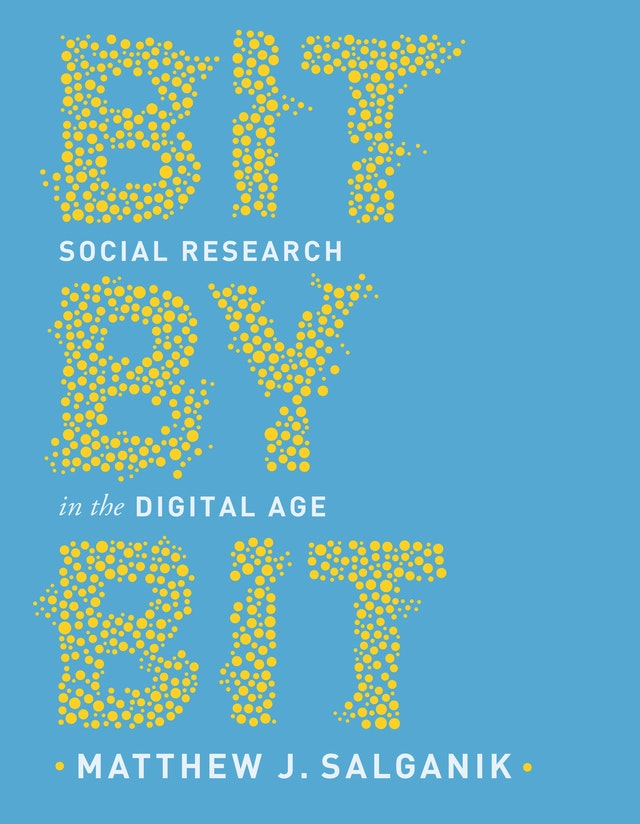
\includegraphics[width=\textwidth]{figures/salganik_bit_2018_cover}
\end{column}%

\hfill%

\begin{column}{.60\textwidth}
1) Introduction \\
2) Observing behavior \\
3) Asking questions \\
4) Running experiments \\
5) Mass collaboration \\
\textcolor{blue}{6) Ethics} \\
\textcolor{blue}{Part 1}, Part 2, Additions and extensions \\
7) The future \\
\end{column}%
\end{columns}

\end{frame}
%%%%%%%%%%%%%%%%%%%%%%%%%
\begin{frame}

Computational social scientists should care about research ethics
\pause
\begin{itemize}
\item fear-based reasons
\pause
\item hope-based reasons
\pause
\item we have no choice
\end{itemize}

\end{frame}
%%%%%%%%%%%%%%%%%%%%%%%%%%
\begin{frame}

I want you to be able to:
\begin{itemize}
\item design ethically thoughtful research
\pause 
\item explain your decisions to others
\end{itemize}
 
\end{frame}
%%%%%%%%%%%%%%%%%%%%%%%%%%
%\begin{frame}
%
%A note on lectures and readings:\\
%For today, I'm going to repeat some of what is in my book, but going forward, I will assume that you've read the chapter.
%
%\end{frame}
%%%%%%%%%%%%%%%%%%%%%%%%%%
\begin{frame}

Two existing approaches:
\begin{itemize}
\item Rules-based approach
\pause
\item Ad hoc approach
\end{itemize}
\pause
My preferred approach:
\begin{itemize}
\item Principles-based approach
\end{itemize}

\end{frame}
%%%%%%%%%%%%%%%%%%%%%%%%%%
\begin{frame}

\begin{center}
\Large{Three examples}
\end{center}

\end{frame}
%%%%%%%%%%%%%%%%%%%%%%%%%%
\begin{frame}

Examples:
\begin{itemize}
\item \textcolor{blue}{Emotional contagion}
\end{itemize}

\end{frame}
%%%%%%%%%%%%%%%%%%%%%%%%%%%
\begin{frame}

\begin{figure}

\includegraphics[width=\textwidth]{figures/kramer_experimental_2014_title}
\end{figure}

\vfill
\url{https://doi.org/10.1073/pnas.1320040111}
\end{frame}
%%%%%%%%%%%%%%%%%%%%%%%%%%%
\begin{frame}

Examples:
\begin{itemize}
\item Emotional contagion
\item \textcolor{blue}{Tastes, Ties, and Time}
\end{itemize}

\end{frame}
%%%%%%%%%%%%%%%%%%%%%%%%%%%
\begin{frame}

\begin{figure}
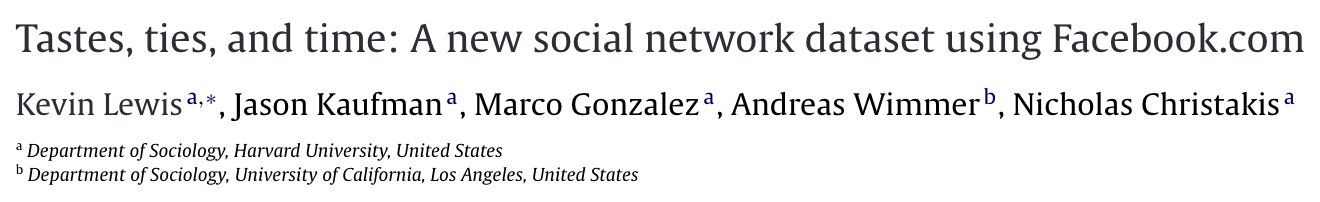
\includegraphics[width=\textwidth]{figures/lewis_tastes_2008_title}
\end{figure}

\vfill
\url{https://doi.org/10.1016/j.socnet.2008.07.002}

\end{frame}
%%%%%%%%%%%%%%%%%%%%%%%%%%%
\begin{frame}

Examples:
\begin{itemize}
\item Emotional contagion
\item Tastes, Ties, and Time
\item \textcolor{blue}{Encore}
\end{itemize}

\end{frame}
%%%%%%%%%%%%%%%%%%%%%%%%%%%
\begin{frame}

\begin{figure}

\includegraphics[width=\textwidth]{figures/burnett_encore_2015_title}
\end{figure}

\vfill
\url{http://dx.doi.org/10.1145/2785956.2787485}

\end{frame}
%%%%%%%%%%%%%%%%%%%%%%%%%%%
\begin{frame}

What's the problem?
\begin{itemize}
\item Increasing power
\pause
\item Inconsistent and overlapping rules, norms, and expectations
\pause
\begin{itemize}
\item Rules are slow to change
\pause
\item Little agreement about key concepts (e.g., privacy)
\pause
\item Blending of contexts
\end{itemize}
\end{itemize}

\end{frame}
%%%%%%%%%%%%%%%%%%%%%%%%%%%
\begin{frame}

\begin{center}
\includegraphics[width=0.9\textwidth]{figures/ethics_schematic_simple.png}
\end{center}

\end{frame}
%%%%%%%%%%%%%%%%%%%%%%%%%%%
\begin{frame}

\begin{itemize}
\item Respect for persons
\end{itemize}

\end{frame}
%%%%%%%%%%%%%%%%%%%%%%%%%%
\begin{frame}

Respect for persons:\\
Participants decide not you

\end{frame}
%%%%%%%%%%%%%%%%%%%%%%%%%%
\begin{frame}

\begin{itemize}
\item Respect for persons
\item Beneficence
\end{itemize}

\end{frame}
%%%%%%%%%%%%%%%%%%%%%%%%%%
\begin{frame}

Beneficence:\\
Minimize risk, maximize benefits, then decide

\end{frame}
%%%%%%%%%%%%%%%%%%%%%%%%%%
\begin{frame}

\begin{itemize}
\item Respect for persons
\item Beneficence
\item Justice
\end{itemize}

\end{frame}
%%%%%%%%%%%%%%%%%%%%%%%%%%
\begin{frame}

Justice:\\
distribution of burdens and benefits of research
\pause
\begin{itemize}
\item poorly education and disenfranchised citizens
\item prisoners
\item institutionalized and mentally disabled children
\item old and debilitated hospital patients
\end{itemize}
\pause
Also includes access to benefits of research

\end{frame}
%%%%%%%%%%%%%%%%%%%%%%%%%%
\begin{frame}

\begin{itemize}
\item Respect for persons
\item Beneficence
\item Justice
\item Respect for Law and Public Interest
\end{itemize}

\end{frame}
%%%%%%%%%%%%%%%%%%%%%%%%%
\begin{frame}

Respect for Law and Public Interest:\\
\begin{itemize}
\item compliance
\item transparency-based accountability
\end{itemize}

\end{frame}
%%%%%%%%%%%%%%%%%%%%%%%%%
\begin{frame}

\begin{itemize}
\item Respect for persons
\item Beneficence
\item Justice
\item Respect for Law and Public Interest
\end{itemize}

\vfill
How do you balance these four principles?

\end{frame}
%%%%%%%%%%%%%%%%%%%%%%%%%
\begin{frame}

\begin{itemize}
\item Consequentialism (focus on ends)
\item Deontology (focus on means)
\end{itemize}
\pause
\vfill
A few things to keep in mind:
\begin{itemize}
\item Both of these approaches can be taken to extremes
\pause
\item Most disagreements are between people taking different approaches 
\end{itemize}

\end{frame}
%%%%%%%%%%%%%%%%%%%%%%%%%
%\begin{frame} {Quick question}
%
%In arguing against the Emotional Contagion experiment (Kleinsman and Buckley, 2015) wrote:
%\begin{quote}
%``Even if it is true that the risks for the Facebook experiment were low and even if, in hindsight, the results are judged to be useful, there is an important principle at stake here that must be upheld.  In the same way that stealing is stealing no matter what amounts are involved, so we all have a right not to be experimented on without our knowledge and consent, whatever the nature of the research.'' 
%\end{quote}
%This argument is rooted in which ethical framework?
%\begin{enumerate}
%\item Consequentialism
%\item Deontology
%\end{enumerate}
%
%\end{frame}
%%%%%%%%%%%%%%%%%%%%%%%%%
\begin{frame}

\begin{center}
\includegraphics[width=0.9\textwidth]{figures/ethics_schematic_simple.png}
\end{center}

\end{frame}
%%%%%%%%%%%%%%%%%%%%%%%%%
\begin{frame}

Applying these ideas can be tricky, in part 2 I will:
\begin{itemize}
\item discuss 4 areas of difficulty
\item offer 3 practical suggestions
\end{itemize}

\end{frame}
%%%%%%%%%%%%%%%%%%%%%%%%%%%
\begin{frame}

\begin{center}
\LARGE
Thank you
\end{center}

\end{frame}
%%%%%%%%%%%%%%%%%%%%%%%%%%%




\end{document}
